\section{Processi primari}

\subsection{Fornitura}
\subsubsection{Rapporti con il Proponente}
Il proponente offre al team diversi canali di comunicazione (mail, discord) attraverso i quali è possibile organizzare una riunione con tempistiche molto brevi. \\
Non ci sono meeting regolari pianificati ma entrambe le parti si mantengono aggiornate con costanza. \\
Tra i motivi di discussione ci sono:
\begin{itemize}
    \item dubbi sulle tecnologie utilizzate;
    \item dubbi su requisiti e vincoli del capitolato;
    \item feedback sul lavoro prodotto (software e documentazione);
    \item tempistiche progettuali;
\end{itemize}
Ognuno di questi meeting è poi riassunto nel verbale corrispondente da un membro del team e verificato da un altro.

\subsubsection{Pianificazione}
La pianificazione è suddiviso in sottosezioni corrispondenti ai scrum.
In ogni scrum sono riportate le seguenti informazioni:
\begin{itemize}
    \item Durata dello scrum
    \item Obiettivi da raggiungere nello scrum 
    \item Attività da svolgere per l'avanzamento
    \item Grafico che illustra le durate previste per le attività
\end{itemize}

\subsubsection{Bilancio}

In questa sezione sono riportati i grafici che descrivono i preventivi e i consuntivi relativi ad ogni periodo di Scrum.\\
Sono state evidenziate in verde le celle che rappresentano le ore produttive usate dai membri del team nei corrispondenti ruoli.\\       
Vengono poi riportati le motivazioni per gli scostamenti verificati e i provvedimenti che verrano adottati attivamente al fine di migliorare l'accuratezza dei preventivi.\\
Inoltre è stato riportato anche il budget totale del progetto fino allo scrum n-esimo nella sezione di riepilogo.\\
Il budget totale preventivato è stato calcolato sommando i costi necessari per lo scrum n-esimo e il budget consuntivo totale dello scrum precedente.\\


\subsection{Sviluppo}

\subsubsection{Scopo}
Lo scopo di questo processo è definire nel dettaglio tutte le procedure da seguire durante lo sviluppo del software, definendo obiettivi, vincoli tecnologici e di design, e test/validazione.

\subsubsection{Attività}
Le attività che prevede il processo di sviluppo sono \textbf{Analisi dei Requisiti}, \textbf{Progettazione} e \textbf{Codifica}.

\paragraph{Analisi dei Requisiti}
Gli analisti del team si occuperanno di sviluppare questo documento (dopo lo studio del capitolato e confronto con il proponente) che dovrà descrivere nel dettaglio le funzionalità principali del prodotto. Nello specifico, il documento dovrà contenere:
\begin{itemize}
\setlength\itemsep{0.1em}
    \item Tecnologie scelte - Intero "stack" con descrizione;
    \item Casi d'uso - Descritti graficamente (tramite diagrammi UML) e testualmente;
    \item Requisiti - Funzionali, Prestazionali, di Qualità;
    \item Vincoli di Progetto.
\end{itemize}

\paragraph{Progettazione}
Durante l'attività di \textbf{Progettazione}, il team dovrà definire una soluzione al problema del capitolato, partendo dallo studio svolto nell'attività \textbf{Analisi dei Requisiti} e quindi da tutto ciò che è stato definito nell'omonimo documento.
\\
Le due parti che compongono questa attività sono:
\begin{itemize}
    \item  \textbf{Requirements \& Technology Baseline} (RTB):
    \begin{itemize}
        \item motivazione delle tecnologie scelte per lo sviluppo software;
        \item stesura di Piano di Progetto, Piano di Qualifica, Norme di Progetto, Verbali;
        \item sviluppo Proof of Concept, un prototipo che dimostri le funzionalità del prodotto;
    \end{itemize}
    \item \textbf{Product Baseline} 
    \begin{itemize}
        \item definizione delle linee guida architetturali del prodotto, basate sulla RTB;
        \item stesura di Manuale utente e Verbali.
    \end{itemize}
\end{itemize}

\paragraph{Codifica}
Durante questa attività si andrà a tradurre in codice tutta la parte che riguarda l'analisi svolta durante le attività precedenti, concretizzando la soluzione software.
Per quanto riguarda lo stile del codice, si adotteranno le seguenti convenzioni:
\begin{itemize}
\setlength\itemsep{0.1em}
    \item Per i nomi delle variabili va utilizzato camelCase (iniziale minuscola).
    \item Il codice va indentato correttamente per favorire la leggibilità.
    \item Le funzionalità vanno separate in file semplici e con scopi unici.
    \item Limitare le dipendenze tra elementi del codice.
\end{itemize}

\subsubsection{WorkFlow Codifica}
Il team ha creato due repository separate da quella principale nelle quali lavorare rispettivamente al lato mobile e web dell'applicativo, ciò permette meno complicazioni di merge e dei commit più "puliti" sulla repo principale (vengono effettuati solo quando sono presenti grandi passi avanti). \\[0.1cm]
Generalmente si è deciso che in ogni periodo o scrum il team verrà suddiviso in due gruppi ai quali sono assegnate le due repository di sviluppo, questo permette ad ogni membro di concentrarsi su singoli aspetti del progetto e facilita la collaborazione essendo i sottogruppi meno numerosi. 
\\[0.3cm]
L'obiettivo principale dei momenti di codifica deve essere la trasformazione in codice eseguibile della progettazione dedotta dai requisiti. Le idee ed il funzionamento devono essere già ben definiti prima di dedicarsi alla scrittura e compilazione. Lavorare a livello più teorico prima di codificare aiuta la produzione di codice più comprensibile e ben pensato perché appunto pianificato totalmente in anticipo.\\
\begin{center}
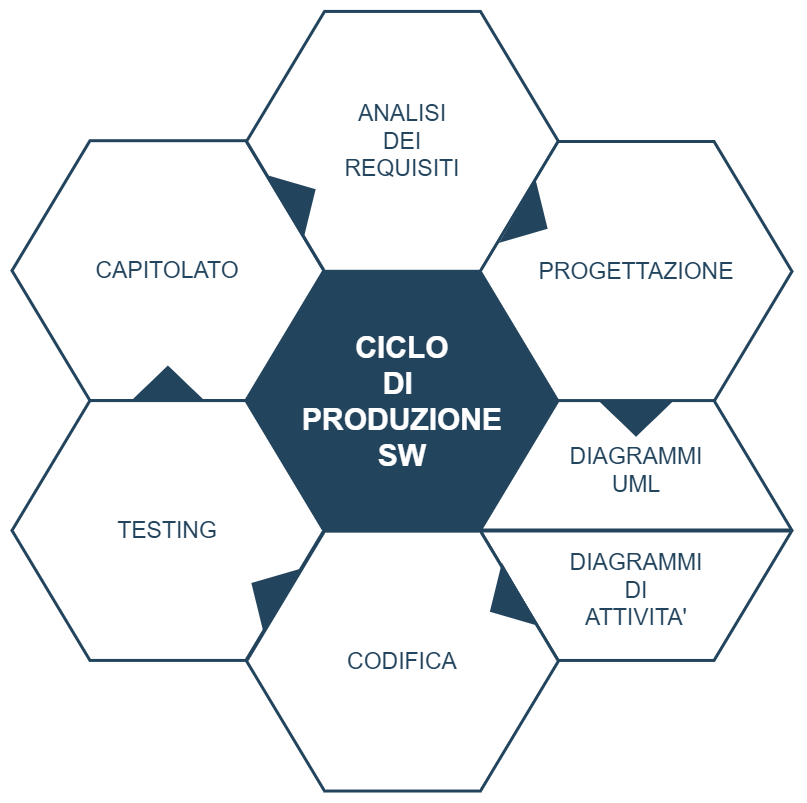
\includegraphics[scale=0.3]{img/scheminoCodifica.png}
\end{center}
Come si può notare dall'immagine precedente la codifica rappresenta uno degli ultimi passaggi del ciclo di produzione, questo perché essa va limitata alla semplice scrittura in codice di idee ben chiare sul funzionamento dell'applicativo.

\subsection{Struttura Codice}
\subsubsection{Best Practice}
\begin{itemize}
    \item Per i nomi delle variabili va utilizzato camelCase (iniziale minuscola).
    \item Il codice va indentato correttamente per favorire la leggibilità.
    \item Le funzionalità vanno separate in file semplici e con scopi unici.
    \item Limitare le dipendenze tra elementi del codice.
\end{itemize}